\documentclass[10pt,a4paper]{report}
\usepackage[utf8]{inputenc}
\usepackage[spanish]{babel}
\usepackage{amsmath}
\usepackage{amsfonts}
\usepackage{amssymb}
\usepackage{graphicx}
\usepackage{fancyhdr}
\usepackage{float}
\usepackage{color}
\usepackage{mcode}
\usepackage[left=2cm,right=2cm,top=2cm,bottom=2cm]{geometry}
%%%%%%%%%

\pagestyle{fancy}
\fancyhf{}
\lhead[]{}
\chead[]{}
\rfoot{\thepage}
\lfoot[]{}
\cfoot[]{}

\renewcommand\headrule
{{\color[RGB]{98,36,35}%
		\hrule height 2pt
		width\headwidth
		\vspace{1.3pt}%
		\hrule height 1pt
		width\headwidth
	}}
	\addto\captionsspanish{\def\tablename{Tabla}}%imprime Tabla en lugar de Cuadro
	%%
	\spanishdecimal{.} 
	

\begin{document}
\thispagestyle{fancy}
%\maketitle
\tableofcontents
\newpage
\setcounter{chapter}{1}
\section[Introducción]{Introducción}

\subsection{Ejercicio 4}
4.-Determine si los siguientes sistemas de tiempo continuo son o no lineales, variantes en el tiempo, causales, con memoria y estables. Justifique su respuesta.
%%
\begin{itemize}
\item \begin{equation}
 y(n)=
 \left\{
  \begin{aligned}
   1\quad n>=0\\
   0\quad n<0\
  \end{aligned}
 \right.
\label{escunit}
\end{equation}
%%
Este no es el modelo de un sistema ya que no relaciona la entrada con la salida.
\item  \begin{equation*}
y(t)=sen(x(t+1))
\end{equation*} 
* Lineal o no lineal\\
   
   x1(t) = y1(t)= sen (x1(t+1))\\
   x2(t) = y2(t)= sen (x2(t+1))\\
   x3(t) = x1(t)+x2(t) = y3(t)=sen(x3(t+1))\\
                         y3(t)=sen(x1(t+1)+x2(t+1))\\
   
 NO LINEAL\\
   
* Variante o invariante en el tiempo\\
	
	y(t-t0)=sen(x(t-t0+1)) ... A esto se debe llegar\\
	Proponer: x1(t)=x(t-t0) --- y1(t)=sen(x1(t+1))\\
	y1(t)=sen(x(t+1-t0))\\
	
	INVARIANTE EN EL TIEMPO\\
	
* Causalidad\\

y(0)=sen(x(1))\\
y(-1)=sen(x(0))\\
y(1)=sen(x(2))\\

NO CAUSAL O ANTICIPATIVO, porque depende de valores futuros. \\

* Memoria\\

CON MEMORIA, por que depende de valores futuros.\\

* Estabilidad\\
ESTABLE, ya que al probar con una señal como el escalón, la entrada y la salida es acotada.\\

\end{itemize}

\subsection{Ejercicio 8}
8.-Capture al menos dos señales físicas reales y preséntelas en una  gráfica e identifique el tipo de señal en algún segmento de la misma.\\

\begin{itemize}
\item La primera señal es un silbido humano.\\
Código de Matlab:\\
\begin{lstlisting}[frame=single]
>> [y,Fs] = audioread('Silb.wav');
>> sound(y,Fs);
>> figure(2);
>> plot(y);
\end{lstlisting}

\begin{figure}[htb]
\centering
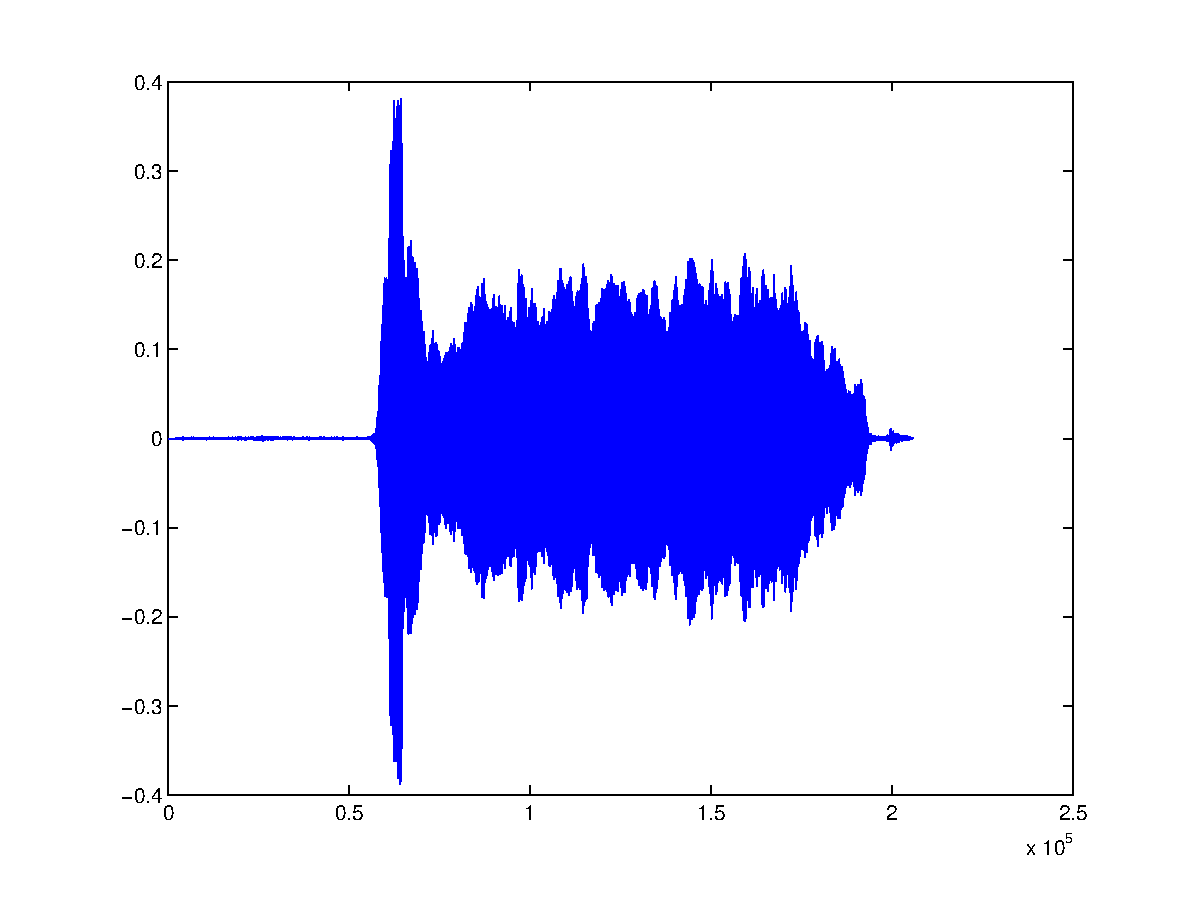
\includegraphics[width=0.6\textwidth]{SilbGraphic}
\caption{Silbido humano}
\label{fig:SilbGraphic}
\end{figure}

Esta es una señal de tiempo continuo por que la señal puede tomar cualquier valor en cualquier instante de tiempo. \\
Es una señal aperiódica, ya que no se repite en intervalos regulares \\
Es una señal aleatoria, ya que no se puede predecir mediante una función matemática.\\
Notamos en la gráfica que la señal el totalmente impredecible, ya que siempre parece tomar diferentes valores de frecuencia.

\item La segunda señal corresponde al sonido de las cuerdas de una guitarra acústica.\\
Código de Matlab:\\
\begin{lstlisting}[frame=single]
>> [y,Fs] = audioread('Guitar.wav');
>> sound(y,Fs);
>> figure(1);
>> plot(y);
\end{lstlisting}

\begin{figure}[H]
\centering
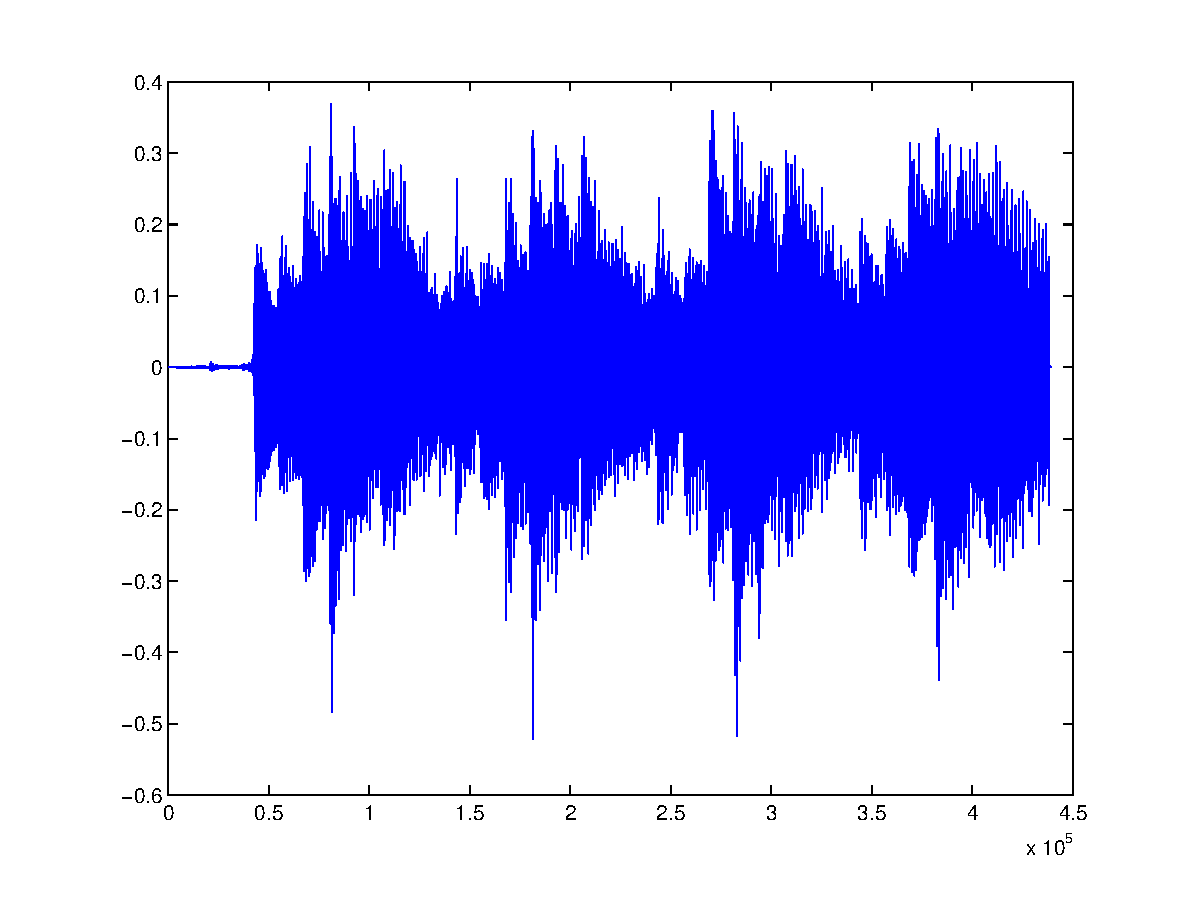
\includegraphics[width=0.6\textwidth]{GuitarGraphic}
\caption{Sonido de las cuerdas de una guitarra acústica}
\label{fig:GuitarGraphic}
\end{figure}

Esta es una señal de tiempo continuo por que la señal puede tomar cualquier valor en cualquier instante de tiempo. \\
Es una señal aperiódica, ya que no se repite en intervalos regulares \\
Es una señal aleatoria, ya que no se puede predecir mediante una función matemática.\\
NOTA: Se trató de que el rasgeo de las cuerdas de la guitarra sean igual en tiempo e intensidad, resultó un poco difícil, el mejor de los casos qes que hubiera salido igual la gráfica en intervalos regulares, para que la señal sea periódica y determinística. 

\end{itemize}

\end{document}
